\chapter{Background}
\label{chapter:chapter02}

This chapter presents a review of the literature for the considered single-objective algorithms and multi-objective algorithms. It also defines important concepts to understand the results produced, such as the concept of optimisation and dominance. After, it introduces the metrics that help compare the different approaches. Finally, it explains the criteria considered for preference prediction.

\section{Optimality}

There are two interpretations of optimality. One refers to single-objective optimisation and the other to multi-objective optimisation.\\

\subsection{Single-Objective Optimisation}

An optimisation problem refers to find the solution that gets the minimum or maximum value of a given function $f(x)$, subject to a set of constraints. Mathematically, it can be stated as follows:\\
 
 \begin{equation}
     \begin{aligned}
     \min & f\left( \vect{x_i}\right)\\
     \text{subject to } & g_i\left( \vect{x_i}\right) \leq 0\\
     & h\left( \vect{x_i}\right) = 0\\
     x_i \in \Omega
     \end{aligned}
 \end{equation}
 
\noindent where $\vec{x} = (x_1,...,x_n)$ is an $n$-dimensional decision variable vector, $g_i(x_i)$ and $h_j(x_i)$ refer to the set of constraints that must be fulfilled while optimising $f(x_i)$, and $\Omega$ is the universe representing all the acceptable solutions possible that can be used to satisfy $f(x_i)$ and its constraints. The $\vec{x}$ decision vector can be whether continuous or discrete variables and its evaluation can also be continuous or discrete.\\

\begin{definition}
    Single-objective global optimisation is defined as given a function $f: \omega \subseteq \mathbb{R}^n \rightarrow \mathbb{R}, \Omega \neq \emptyset$ for $x_i \in \Omega$ the value $f^* \triangleq f(\vec{x}^*) > -\infty$ is called a \textbf{global minimum} if and only if\\
    
    \begin{equation}
        \forall x \in \Omega: f(\vec{x}^*) \leq f(x).
    \end{equation}
\end{definition}

$\vec{x}^*$ is by definition the global minimum solution. The goal of determining the global minimum solution is called the \textbf{global optimisation problem} for a single-objective problem.\\

\subsection{Multi-Objective Optimisation}

Optimisation problems that involve two or more objectives are
known as multi-criteria or multi-objective optimisation problems (MOPs).
In MOPs, objectives are usually in conflict, this means that it is not possible to compare two solutions $\vec{x}$ and $\vec{y}$ directly, as there is no single solution that would simultaneously be the best for all objectives. The quality of the solutions is therefore compared by their dominance.\\

\begin{definition}
    The \textbf{Dominance} of a solution $a_i$ of a set $A = (a_1,...,a_n)$ is said to \textit{dominate} a solution $b_i$ of another set $B = (b_1,...,b_n)$, denoted by $a_i \preceq b_i$ or $f(a) \preceq f(b)$ with, if and only if $a_i$ is at least as optimal as $b_i$ in all objectives of $b_i$ and with at least one of its objectives better than $b_i$ \cite{back1997handbook}.
\end{definition}

In multi-objective optimisation, the goal is to find the set of optimal solutions, known as the \textbf{Pareto Optimal Set}. Pareto optimality is defined concerning the concept of non-domination between the points of the objective space $\Omega$ if and only if there is no vector in the set $A$ that results better in set $B$.

\begin{definition}
    A \textbf{Pareto Optimal Set} (POS) is composed of optimal solutions, which its internal objectives cannot be improved simultaneously. Formally defined as:
    \begin{equation}
        \mathrm{POS}:=\left\{\mathrm{x}^{*} \in \mathcal{X}: \nexists \mathrm{x} \in \mathcal{X} \subset \mathbf{R}^{n}, \mathrm{x} \prec \mathrm{x}^{*}\right\}
    \end{equation}
\end{definition}  

\begin{definition}
    The \textbf{Pareto Optimal Front} (PF) is the corresponding objective space of vectors from the \textbf{Pareto optimal set} termed as \textit{non-dominated}. This collection of Pareto optimal solutions being the result of the same MOP, where: 
    
    \begin{equation}
        PF^* := \{u= F(x) | x \in P^*\}
    \end{equation}
\end{definition}

\section{Evolutionary Algorithms}

Evolutionary algorithms (EAs) are stochastic optimisation techniques inspired by Darwin's theory of evolution. An EA uses mechanisms inspired by biological evolution such as reproduction, mutation, recombination, and selection. The candidate solutions for optimisation are part of a population, and a fitness function determines the quality of each of these solutions. This fitness takes part after different iterations or generations in which it is sought to get as close as possible to the global optimum~\cite{eiben2003introduction}.\\

Based on this fitness, the best candidates are more likely to be chosen as the parents for the next generation by applying recombination and mutation operators. Recombination is an operator that produces new candidates (children) solutions by combining the genetic information of two or more selected candidates (parents). A mutation operation applies small changes to a solution. Executing recombination and mutation leads to a set of new candidates (the offspring) that compete based on their fitness for a place in the next generation. This process is then iterated until a stop criterion is met.\\

%In this process, two fundamental steps form the basis of evolutionary systems:

%\begin{itemize}
%    \item \textbf{Variation operators} (recombination and mutation) create the necessary diversity and therefore facilitate the possibility of finding new solutions.
%    \item \textbf{Selection} acts as a force that pushes quality.
%\end{itemize}

EAs have several characteristics that can help position themselves within the families of generation and testing methods:

\begin{itemize}
    \item They are population-based, this means that they process a variable number of candidate solutions simultaneously.
    \item They usually use a recombination to inherit the information of more candidates in new solutions.
    \item These algorithms are stochastic.
\end{itemize}

The main components of an EA are listed below:

\begin{itemize}
    \item Representation (definition of solutions).
    \item Evaluation function.
    \item Population.
    \item Parent selection.
    \item Variation, recombination and mutation operations.
    \item Survivor selection mechanism.
\end{itemize}

The above mentioned components are defined to a particular problem. When solving a problem, EAs usually perform the following steps:\\

\begin{itemize}
\item \textbf{Initialisation}: A population of individuals (solutions) is generated at random.
\item \textbf{Evaluation}: Individuals are evaluated using the fitness functions.
\item \textbf{Termination}: A criterion to determine whether the algorithm should stop or not.
\item \textbf{Selection}: Select the solutions that survive to the next generation.
\item \textbf{Variation}: This step can combines the information of two or more individuals to produce a new offspring solutions through a crossover operator. Mutation operation, conversely, changes the genetic information for a single individual.
\end{itemize}.\\

\section{Single-Objective Optimisation Algorithms}

This section describes the different single-objective optimisation algorithms (SOAs) that will be used for the comparison.

\subsection{Local Search}
 
Local Search (LS), also referred as Hill Climbing in maximisation problems and Steepest Descent in minimisation problems, is a SOA based on the idea of generating random starting solutions. Then, at each generation, LS generates the starting solution for the next iteration by perturbing the local optimum found thus far.\\

It is worthy to mention that the perturbing mechanism is an important feature of LS. A weak perturbation may not be enough to escape the local optimum. Conversely, a too strong perturbation may make the algorithm too similar to a multi-start LS with randomly generated starting solutions. A pseudo-code for this algorithm can be seen in Algorithm~\ref{local_search_alg}.\\

\begin{algorithm}[H]
\caption{Local Search Algorithm} 
\label{local_search_alg}
\SetAlgoLined 
 Choose, at random, an initial solution $s$ in the search space\;\\
 Apply a search starting from $s$ to get a solution $s*^$\;\\
 \Repeat{the stopping criterion is satisfied}{
  Perturb $s^*$ to get a solution $p$\;\\
  Apply search starting from $p$ to get a solution $p*$\;\\
  \eIf{the acceptance criterion is satisfied}{
   $s^*$ \gets $p^*$\;
  }
 }
 \textbf{return} the best solution met\;
\end{algorithm}


\subsection{Genetic Algorithms}

Genetic Algorithms (GAs) were developed in the early 70s in Michigan by J. Holland and his students, who were researching adaptive systems at the time \cite{goldberg1988genetic}.
The definition can be very generic and most of their parts are usually implemented differently according to each problem. Their essential parts include a representation of the solution, a selection strategy, evolutionary operators, and a mutation operator.\\

In  GAs, the binary string is the most common representation. For a binary representation, the mutation is performed by doing a bit-flip in a gene.  Conversely, the crossover operator recombines the genes of two or more individuals, by exchanging half of the information from one parent and a half from the other one. \\

%An external parameter known as $pc$ (crossover rate) indicates the probability of each individual to undergo crossover, this value ranges from $0.6$ to $1.0$ \cite{boussaid2013survey}.\\

%Individuals that can produce offspring are then chosen using a selection strategy after the fitness of each individual has been evaluated. The most common selection scheme is the roulette-wheel selection, but other types of selections such as tournament selection and ranking selection are also common \cite{goldberg1988genetic}.\\

%After the crossover, the offspring are subjected to mutation. This mutation procedure introduces some kind of randomness which in essence introduces new genes in the solution, this is to prevent being trapped into the local optima. This operator is usually used with a small probability, as low as $1/n$ \cite{boussaid2013survey}, but the appropriate mutation rate is still an open issue.\\

Finally, the replacement or survivor selection uses the fitness value to identify the individuals for the next generations and is responsible to assure the survival of the fittest individuals. An example of an implementation of a GA can be seen in Algorithm~\ref{genetic_alg}. \\

\begin{algorithm}[H]
\caption{Genetic Algorithm}
\label{genetic_alg}
\SetAlgoLined 
Generate Initial population $p$\;\\
Compute fitness of each individual\;\

\Repeat{stopping condition has been met}{
    \Comment{Produce a new generation}\;\\
    \For{size of $p$ / 2}{
        Select two individuals from the previous generation for matching\;\\
        Recombine the two individuals to give two new off springs\;\\
        Insert the offspring in the new generation\;\\
    }
}
 \textbf{return} the best solution met\;
\end{algorithm}

\subsection{Evolution Strategies}

Similar to the GAs, Evolution Strategies (ES) follow the principles of natural evolution as their method to solve optimisation problems. They were introduced during the 70s by Rechenberg~\cite{huning1976evolutionsstrategie} and further developed by Schwefel~\cite{back1991survey}. The first algorithm used in experimentation was two-membered ES and had a simple mutation-selection scheme.\\

The basic structure consists of a single parent which produces an offspring following a normally distributed mutation resulting $\lambda$ children. Next, a selection operator determines the fittest individual which then becomes the parent of the next generation.\\

%The selection process resembles a \textit{extinction of the worst}, which means the fewer fit individuals are replaced, which sometimes may include the parents, the population is kept with the size $\lambda$ constantly in each of the generations.\\

%At the time of its conception, the idea of a population was not widely used so far, which is why 
Later, Rechenberg proposed a multi-member ES~\cite{huning1976evolutionsstrategie}, where more than one parent can participate in the generation of one offspring individual. This is denoted as $(\mu + 1)$-ES where $\mu$ represents the number of parents. Two other definitions were then introduced by Schwefel~\cite{reynolds2003effects}, which were $(\mu + \lambda)$-ES and $(\mu, \lambda)$-ES.\\

\begin{itemize}
    \item $(\mu + \lambda)$-ES, known as elitist evolution strategy, indicates that $\mu$ parents will create $\mu \geq 1$ descendants by recombination and mutation, keeping the fittest individual of the previous generation and discarding the rest.
    \item $(\mu, \lambda)$-ES, known as non-elitist evolution strategy, is similar with the difference that none of the parents is kept in any of the subsequent generations, disregarding how good or bad was its fitness compared to the generation they belong.
\end{itemize}\\

%Two other well-known ($ES$) is $(\mu/\rho + \lambda) - ES$ and ($\mu/\rho, \lambda) - ES$, where the $\rho$ refers to the number of parents involved in the procreation the offspring. Mutation in ES can be realised through normally distributed numbers with a mean zero and a standard deviation of $\sigma$, which represents the size in the mutation step when the problem has a continuous solution. A basic version of the ($ES$) can be seen in \ref{evolution_alg}

\begin{algorithm}[H]
\caption{Evolution Strategy Algorithm}
\label{evolution_alg}
\SetAlgoLined
    \textit{Initialise} the population with random individuals\;\\
    \textit{Evaluate} each individual
    \Repeat{the termination condition is satisfied}{
        \textit{Select} parents\;\\
        \textit{Recombine} pairs of parents\;\\
        \textit{Mutate} the resulting offspring\;\\
        \textit{Evaluate} new individuals\;\\
        \textit{Select} individuals for the next generation\;\\
    }
\end{algorithm}

\subsection{Random search} 

Random Search (RS), also known as Pure RS, was first defined by Brooks~\cite{10.2307/167616} and later named in the classic volumes by Dixon and Szeg{\"o}~\cite{doi:10.1002/zamm.19790590220}. RS is considered as one of the most basic search strategies, and it consists of the following:

\begin{itemize}
    \item It creates a new random solution
    \item The best solution is updated if the new solution outperforms the fit value of the previous best solution.
\end{itemize}

While this algorithm sacrifices the guarantee of determining the optimal solution within a given error, it can be shown that RS converges to the global optimum with a probability one \cite{zabinsky2013stochastic}. It is commonly used to compare the performance of other search algorithms to random sampling~\cite{de2017james}.

\subsection{Random Descent} 

Random Descent (RD), also known as Stochastic Hill climbing, is an algorithm similar to regular Hill Climbing. However, RD includes a neighbourhood, which limits the search to only the solutions that are close to the current best solution at each step. The most popular RD implementation was done by Forrest and Mitchell, naming it Random Mutation Hill Climbing (RMHC)~\cite{mitchell1994will}.\\

The local improvements are determined by a neighbourhood structure, which can be seen as an undirected graph G on vertex set S, and a fitness function on the search space of the algorithm. The algorithm checks a member of its neighbourhood randomly and transitions to this solution when there is an improvement in the fitness function result or is the same. The process is then repeated at each step.%\\
%
%It was designed with discrete domains in mind, since they have explicit neighbourhoods, such as with combinatorial optimisation problems. However, even being a stochastic optimisation process, it can still get stuck in a local optimum. 
Algorithm~\ref{evolution_alg} describes the pseudocode for RD.

\begin{algorithm}[H]
\caption{Pseudocode for stochastic hill climbing}
\label{evolution_alg}
\SetAlgoLined
    Currrent solution $s$ from new population\;\\
    Evaluate the objective function $f(s)$\;\\
    $stop = \textit{FALSE}$\;\\
    $iter = 0$\;\\
    \While{$stop = \textit{FALSE}$}{
      Choose a random solution in the neighbourhood $s_n$\;\\
      \eIf{$f(s_n) > f(s)$}{
        replace $s$ by $s_n$\;
       }{
        $iter = iter + 1$\;
      }
      \eIf{$iter = iter_{max}$}{
        $stop = TRUE$\;
      }
     }
\end{algorithm}

\subsection{Parallel Tempering (Replica Exchange Monte Carlo)} 

Parallel Tempering (PT), also known as Replica Exchange Monte Carlo, consists in replicas of a system of interest were simulated at a series of different temperatures. Then, these replicas undergo a partial exchange of configuration information. The more general form of PT with a complete exchange of configuration information was introduced in 1991 by Geyer~\cite{B509983H}. \\

This algorithm runs several replicas of a particular system of interest, using different temperatures in each one of them. High temperature can generate large volumes of phase spaces, while low-temperature systems tend to have more precision in the sampling of the phase space and tend to be trapped in a local optimum. \\

Using this algorithm requires a minimum and maximum temperature, with each replica of the system with an assigned temperature. After each step, the replicas are ordered according to their temperature, and then swapped to push the better solutions to the lowest temperatures, so they can eventually converge while higher temperature replicas are constantly modified in a search for improvement. Each of the replicas applies repeatedly a series of moves to a private solution, and then the global solution is tracked in the main search. The pseudocode for this algorithm can be seen in Algorithm~\ref{parallel_temp_alg}.\\

\begin{algorithm}[H]
\caption{Parallel Tempering}
\label{parallel_temp_alg}
\SetAlgoLined
\For{$i \gets 0$ \textbf{to} $M - 1$}{
    $T_i \gets$ calculate temperature $i$\;\\
    $replica_i \gets$ new instance of Metropolis search with temperature $T_i$
}
\Repeat{The stop criterion has been met}{
    \For{$i \gets 0$ \textbf{to} $M - 1$}{
        Run $replica_i$ for $N_{swap}$ iterations
    }
    $G \gets min(Cost({global_best}_{replica(0)},...,Cost({global_best}_{replica(M - 1)})))$\;\\
    $j \gets U\{0,M-1\} \Comment{Randomly select adjacent temp. levels}$\;\\
    $\Delta E \gets (Cost({active\_solution}_{replica(j)}) - Cost({active\_solution}_{replica(j + 1)}))/G$\;\\
    $\Delta \beta \gets 1/{T_j} - 1/{T_{j+1}}$\;\\
    \eIf{$U(0,1) < min(1,exp(\Delta E\Delta \beta))$}{
        Set the temp. of $replica_j$ and $replica_{j+1}$ to $T_{j+1}$ and $T_j$, respectively\;\\
        $swap($replica_j$,$replica_{j+1}$)$ \Comment{Keeps replicas ordered by temp.}
    } 
}
\end{algorithm}

\section{Multi-Objective Algorithms}

This section describes the different Multi-Objective Optimisation Algorithms (MOAs) that will be used for the comparison.


\subsection{Multi-objective Random Search}

Multi-objective RS is a probabilistic algorithm that serves mostly as an algorithm to benchmark other optimisation algorithms in the literature \cite{zitzler1998multiobjective}. Just like its single objective counterpart, this produces a random set of solutions in each step. The output of the algorithm is the Pareto-optimal set of all solutions generated.

\subsection{Electrostatic Potential Energy Evolutionary Algorithm}

Electrostatic Potential Energy Evolutionary Algorithm (ESPEA) \cite{teich2001pareto} is an algorithm that generates several Pareto front approximations, focusing only on the solutions that appear interesting to the decision-maker. Proposed in \cite{teich2001pareto} after noticing that many of the algorithms found in the literature make use of popular crowding distance metrics that do not necessarily converge into optimality \cite{deb2002fast}. %It also has been shown that an optimal distribution depends on the chosen reference point, but these methods are not adequated for constrained problems or discontinuous Pareto fronts \cite{shukla2014theoretical}.\\
%
The algorithm attempts to design an electromagnetism inspired heuristic, where each solution has an assigned charge based on how close it is to a randomly selected subset from an archive of non-dominates solution. Then, the charges are translated to force vectors, which move the solutions in the search space. The best solutions are stored in an archive that uses clustering and crowding distance to prune the solutions.\\

\begin{algorithm}[H]
\label{espea_alg}
\caption{ESPEA}
\SetAlgoLined
\Begin{
    Generate initial population $P$\;\\
    Copy all non-dominated solutions in $P$ to archive $A$\;\\
    \Repeat{stop criterion has met}{
        Generate a single new solution \textbf{$p$}\;\\
        Remove all solutions from $A$ dominated by $p$\;\\
        \eIf{$\textbf{p} \nsucc \textbf{a} \wedge \textbf{f(p)} \neq \textbf{f(a)} \forall \textbf{a} \in A$}{
            \eIf{$|A| < N$}{
                $A:= A \cup {p}$
            }{
                Calculate $e(a)$ for all $a \in \A$\;\\
                Calculate $e:= (e_{a^1}(p),...,e_{-a^N}(p))$\;\\
                $update(A,p,e)$
            }
        }
    }
}
\textbf{return $A$}
\end{algorithm}

% where e represents the energy

\subsection{Many Objective Metaheuristic Based on the $R2$ indicator}

Many Objective Metaheuristic Based on the $R2$ indicator (MOMBI2), introduced first by Hernandez Gomez and Coello Coello \cite{hernandez2015improved}. It has an advantage over other many-objective optimisation algorithms found in the literature, as a lot of them relies on non-dominated sorting and crowding distance, which can become inefficient as the number of objectives grows. 

%The first version of MOMBI had the problem that it presented a loss of diversity in the solutions as the dimensions of the problem grew \cite{gomez2013mombi}. To address this problem, ($MOMBI2$) uses the Achievement Scalarizing Function (ASF) instead of the Chebyshev function $CHE$, which is similar but introduces normalisation.\\

The $R2$ indicator was introduced by Hansen and Jaszkiewicz~\cite{trautmann2013r2}. The $R2$ indicator compares two sets of points being a reference Pareto front and the approximation of the front. %There are several variants of the $R$ indicator, mainly distinguished by the way utility functions are evaluated and combined.
%
%\begin{itemize}
%    \item $R1$, based on the ratio of the set is better than the other
%    \item $R2$, based on the mean difference in utilities
%    \item $R3$, based on the mean relative difference of in utilities
%\end{itemize}
%
%In particular, the $R2$ definition has been broadly used and is one of the most recommended performance indicators \cite{hansen1994evaluating}. Along with Hypervolume and it is highly correlated to it \cite{hernandez2015improved}. 
MOMBI2 uses $R2$ because it induces the complete ranking in the set of all approximations. It is based on the assumption that it is allowed to add values of different utility functions in the set. Therefore, it is also dependent on the scaling of its utility functions. %The algorithm works as follows, each iteration new individuals are created from the parents selected randomly, looking for those individuals that minimised $ASF$. \\
%
%The maximum values of each objective function constitute a point $zmax$, it is ensured that there are not repeated individuals and the size of the population is at least the desired size, if these requirements are not satisfied, then the $zmax$ point is penalised by updating it with the worse values of the whole population. \\
%
%In the following steps, the population is ranked and then reduced to the desired size.
Algorithm~\ref{mombi2_alg} describes MOMBI2.

\begin{algorithm}[H]
\label{mombi2_alg}
\caption{MOMBI2}
\SetAlgoLined
\textbf{Require:} MOP, stopping criterion,set of weight vectors $W$\;\\
\textbf{Ensure:} Pareto set approximation\;\\
Initialise population $P_i,i \gets 1$\;\\
Evaluate population $P-i$\;\\
Calculate the $L_2-norm$ of objectives for $P_i$\;\\
Set $\vec z^{min} \gets \vec z^*$ and $\vec z^{max} \gets \vec z^{nad}$\;\\
\While{termination condition is not fulfilled}{
    Perform parent selection\;\\
    Generate offspring $P_i'$ using variation operators\;\\
    Evaluate population $P_i'$\;\\
    Calculate the $L_2-norm$ of objectives for $P_i'$\;\\
    Normalize objective functions for $P_i \cup P_i'$\;\\
    Execute $R2$ ranking algorithm $(P_i \cup P_i',W)$\;\\
    Reduce population $P_{i+1} \gets \{P_i \cup P_i'\}$\;\\
    Update reference points $(\vec z^{min},\vec z^{max},P_{i+1},m)$\;\\
    $i \gets i + 1$
}
\textbf{return} $P_i$
\end{algorithm}

% There are the algs. for updating the reference points and the R2 rankings in https://sci-hub.se/10.1145/2739480.2754776, but I'm not sure if they should be included here.

\subsection{Non-dominated Sorting Genetic Algorithm II}

Non-dominated Sorting Genetic Algorithm II (NSGA-II), proposed by Deb et al.~\cite{deb2002fast}, makes use of the Crowding Distance which is a certain preference for solutions that are less crowded in the solution space.\\

This algorithm works as follows. After an initial population is created, each individual is ranked and sorted according to their non-dominance level, each solution then is assigned a fitness according to their non-domination level (1 is assigned to the best, then 2 and so on). Then a binary tournament selection, crossover and mutation take place and an offspring population of equal size is created. The process is then repeated joining the previous generation and their offspring as the same population, and it continues with the population always taking the parents of the previous generation; therefore, elitism is ensured. It is important to notice that in the following generations, the ranking will also consider the crowding distance. The pseudocode for this algorithm can be seen in Algorithm~\ref{nsgaii_alg}.

\begin{algorithm}[H]
\caption{NSGAII}
\label{nsgaii_alg}
\SetAlgoLined
Generate a random initial population $P_t$\\
$R_t \gets P_t \cup Q_t$ \Comment{combine parent and offspring population}\\
$F \gets fast-non-dominated-sort(R_t)$ \Comment{run the fast non dominates sort procedure and collect $F = (F_1,F_2,...)$ with the non-dominated fronts of $R_t$}\\
$P_{t+1} = 0$ and $i = 1$\\
\Repeat{$|P_{t+1}| + |F_i| \leq N$ \Comment{until the parent population is filled}}{
    $crowding-distance-assigment(F_i)$ \Comment{calculate crowding-distance in $F_i$}\\
    $P_{t+1} = P_{t+1} \cups F_i$\\
    $i = i + 1$
}
$Sort(F_i, \prec_n)$\\
$P_{t+1} = P_{t+1} \cups F_i[1:(N-|P_{t+1}|)]$\\
$Q_{t+1} = make-new-pop(P_{t+1})$\\
$t = t+1$\\
\end{algorithm}

\subsection{Strength Pareto Evolutionary Algorithm 2}

Strength Pareto Evolutionary Algorithm 2 (SPEA2) \cite{zitzler2001spea2}, first introduced by Zitzler and Thiele in 1999, was among the first techniques that were extensively compared to several existing evolution-based methods \cite{coello2007evolutionary}.\\

SPEA2 makes use of an external non dominated set. For each individual in this set, a strength value is computed, which consist of the raw fitness value assigned from the objective functions and a density estimation similar to the ranking value of MOGA~\cite{fonseca1993genetic}. The algorithm applies the respective selection, crossover and mutation operators to fill an archive of individuals, then applies this fitness function and the non-dominated individuals from both the original population and the archive are copied into a new population. If the number of non-dominated individuals is greater than the population size, a truncation operator based on the distance to the k-nearest neighbour is used. Hence, the individuals having the minimum distance to every other are discarded. Pareto dominance is used to ensure that the solutions are properly distributed along the Pareto front. SPEA2 differs from its predecessor SPEA in three ways: \\ 

\begin{enumerate}
    \item \textbf{Considering the fitness assignment}, the individuals that are dominated by the same archive members have identical fitness values. That means, in case that the archive has only one individual all population members will have an independent rank value, therefore lowering the selection pressure and making SPEA behave like a random search algorithm.
    \item \textbf{For the density estimation}, if many individuals are indifferent to the current generation, which means there is no domination between them, there is little to no information that can be obtained from them, which happens rather frequently, density information is used to guide the search more effectively. Clustering makes use of this information but only regarding the archive and not the population.
    \item \textbf{Archive Truncation}, considers that, while in SPEA the clustering technique was able to reduce the non-dominated set, without destroying its features, it could lose outer solutions, however, these solutions must be kept in the archive to keep the spread of non-dominated solutions.
\end{enumerate}

%The algorithm works as follows. First, all non dominated members are copied to the archive, if there is any dominated individual or a duplicate (with the same objective function evaluation), then they are removed from it during the update operation. If the size of the updated archive exceeds the predefined limit, further members are removed by a clustering technique which preserves the features of the non-dominated front.\\

Then the fitness values are assigned to the archive and the population members. 
\begin{itemize}
    \item Each individual $i$ is assigned a strength value $S(i) \in [0, 1)$, which  at the same time considers the fitness function $F(i)$. $S(i)$ is the number of population members $j$ that are dominated or equal to i, divided by the population plus one.
    \item The fitness $F(j)$ of an individual $j$ in the population is calculated by summing the values of $S(i)$ of the rest of the archive members that dominate or are equal to $j$ plus one.
\end{itemize}

Then for the mating selection, individuals are selected by binary tournaments. This assumes a minimisation, each member of the archive has a higher chance of being selected than the rest of the population. Finally, after crossover and mutation operators are applied, the population is replaced by the resulting offspring population. The pseudocode for this algorithm can be seen in Algorithm~\ref{spea2_alg}.\\

\begin{algorithm}[H]
\caption{SPEA2}
\label{spea2_alg}
\SetAlgoLined
\textbf{Input:} \textit{population size} $N$, \textif{archive size} $\bar N$, \textit{maximum number of generations} $T$\;\\
\textbf{Output:} \textit{nondominated set} \textbf{A}\;\\
\textit{Initialize:} Generate an initial population $P_0$ and create the empty archive $\bar P_o = 0.$ Set $t = 0$\;\\
\Repeat{$t \leq T$ or any stopping criterion is satisfied.}{
    \textit{Fitness assignment:} Calculate fitness values of individuals in $P_t$ and $\bar P_t$\;\\
    \textit{Environmental selection} Copy all nondominated individuals in $P_t$ and $\bar P_t$ to $\bar P_{t+1}$. \;\\
    \eIf{$size(\bar P_{t+1}) > \bar N$}{
        \textit{Reduce} $\bar P_{t+1}$ by means of the truncator operator
    }{
        \textit{Fill} $\bar P_{t+1}$ with dominated individuals in $P_t$ and $\bat P_t$
    }
}
\textit{Termination:} $A \gets$ the set of decision vectors represented by the nondominated individuals in $\bar P_{t+1}$\;\\
\textit{Mating selection:} Perform binary tournament selection with replacement on $\bar P_{t+1}$ in order to fill the mating pool.
\end{algorithm}

\section{Comparing Single-Objective and Multi-Objective Optimisation}

%REWRITE
H. Ishibuchi et al.~\cite{Ishibuchi_single_vs_multiobjective} presented a general study of this topic. The experiments are related to the comparison of single-objective GAs (SOGA) and multi-objective GAs (MOGA). In this work is also discussed the several difficulties occurring when comparing both types of algorithms, such as the inability to use hypervolume (HV) as a comparison metric, since it strongly depends on the location of the origin.\\

Different works include a comparison between single-objective and multi-objective strategies for different fields of the industry \cite{mehboob2016genetic,leal2018aero,shiau1994multiobjective}. For example, Jiao and Zeng \cite{Jiao2017DynamicME} among others make use of different strategies to convert a mono-objective problem into a dynamic multi-objective one in which apply a multi-objective evolutionary algorithm with improved results compared to existing solutions. Another recurring theme in which their performance is compared is in the design of antennas to improve cellular reception, as is the case of the work of Rahmat-Samil and Nanbo Jin. \cite{Jin2007-qu}.\\

Finally, Battiti and Passerini \cite{Battiti2010-xo} talk about the use of GAs that adapt to the decision-maker, this is relevant because in the final platform the user does not properly have a real decision on which group will end up being assigned but this is intended to be done automatically. Battiti mentions some of the possible strategies for adapting the behaviour of a decision-maker and also discusses some of the limitations that such a system would present according to their preferences~\cite{Wang2010-zh}.\\

\section{Metrics}

The next section includes metrics to use for comparison with multi-objective algorithms. The only metric that has shown to represent the domination of a set to another is the HV, however this metric is considered costly as the number of objectives and solutions grows and is usually considered to compare the performance between different algorithms, while the rest of the metrics serve as good approximations of the HV, that require less computational cost and can be calculated in each generation or step to choose a set of solutions over another. Besides there exist other sets of metrics such as spread that measure the distribution of the solutions within a given front, this helps determine the quality of the front because it considers a wider space covered within the search space.\\

\subsection{Hypervolume}

First defined by Zitzler and Thiele \cite{zitzler1999multiobjective}, as:

\begin{definition}
The size of space covered $S$ by a front $X' = (x_1, x_2,...,x_k)$, as a set of points in a Front, then $S(X')$ gives the volume enclosed by the union of the polytopes $p_1, p_2,... p_k$ where each $p_i$ is formed by the intersection of the hyperplanes arising out of ${x_i}$ along with the axes, for each of them in the objective space, there exists a hyperplane perpendicular to this axis and passing thought the point $(f_i(x_i), f_2(x_i), f_n(x_i))$. In the two dimensional case, each $p_i$ represents a rectangle defined by the points $(0,0)$ and $(f_1(x_i),f_2(x_i))$.
\end{definition}\\

HV is considered the only unary indicator that is capable of truly detecting that a front $A$ is not worse than another front $B$ for all its pairs $A\triangleright B $ \cite{zitzler2003performance}.  This concept is referred as \textit{pareto complaint}~\cite{ishibuchi2015study}. It is also noticed that for all the points in a front $A$ and a front $B$, $A \triangleright B $ follows $I_H(A) > IH(B)$, because this means that $A$ must include at least one point that is not weakly dominated by $B$, therefore a portion of the objective space is covered by $A$ but not by $B$.\\

This can be more clearly seen in Figure~\ref{fig:hv_graph}, wherein the former the grey area represents the $HV(S,r)$ in the search space.\\

\begin{figure}
    \centering
    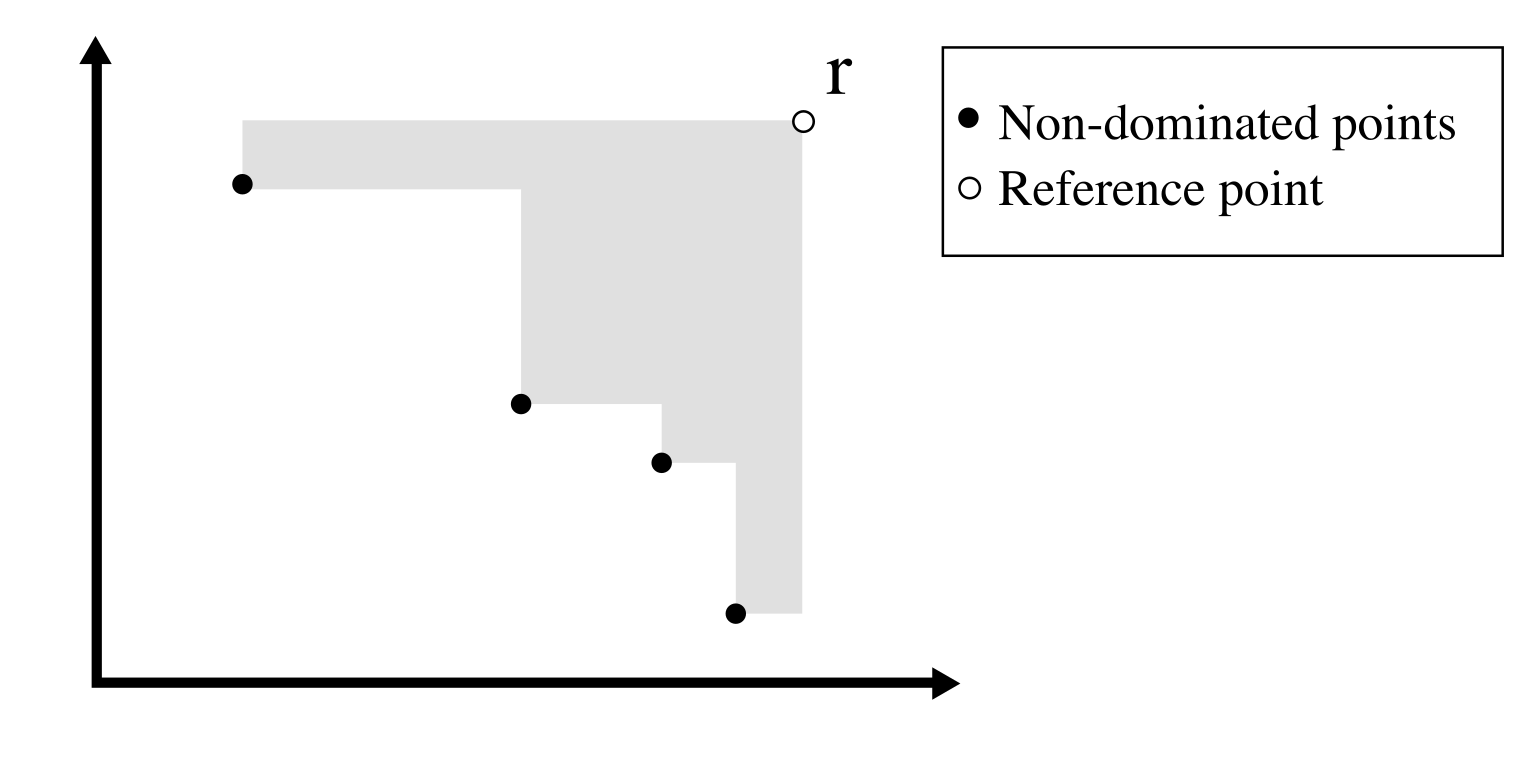
\includegraphics[width=0.5\textwidth]{images/hv_graph.png}
    \caption{Demonstration of the (HV) in two dimensions, the grey area represents the value of $HV(S,r)$}
    \label{fig:hv_graph}
\end{figure}

One more general definition can be found in \cite{audet2018performance} where it is described as the volume of the space in the objective space dominated by an approximation of the Pareto Front $S$ and delimited from the above by a reference point $r \in R^{m} $, so, for all the points $z$ in the obtained front. The hyper-volume is given by:

\begin{equation}
H V(S, r)=\lambda_{m}\left(\bigcup_{z \in S}[z ; r]\right)
\end{equation}

Where $\lambda_m$ is the $m-$dimensional Lebesgue measure.\\

One of the major drawbacks of using HV is that its complexity results in $\mathcal{O}(|S|^{m/2}log|S|)$ and is also the main reasons other measurements are preferred over HV especially in many-objective problems. It has been used without issues with the number of objectives lower than 10 and a non-dominated number of solutions less than 10000. However other methods and algorithms have been proposed to address this issue \cite{audet2018performance}.

\subsection{Spread}

First defined by Deb et al. in \cite{zitzler2003performance}, the metric spread often represented as $\bigtriangleup$. It measures the extent of spread achieved among the obtained solutions. Its goal is to get a set of solutions that spans the entire Pareto-optimal region.

The euclidean distance $d_i$ is calculated between each consecutive solution in and obtained front. Then the average $\overline{d}$ is calculated for these distances, so for a front composed of non-dominated solutions, first the extreme solutions of the objective space are obtained, these are considered the boundaries of the obtained solutions, this is done by fitting a curve parallel to the Pareto front. Afterwards, the spread is calculated using Equation~\ref{eq:spread_eq}.\\

\begin{equation}
\Delta=\frac{d_{f}+d_{l}+\sum_{i=1}^{|N D S|-1}\left|d_{i}-\bar{d}\right|}{d_{f}+d_{l}+(|N D S|-1) \bar{d}}
\label{eq:spread_eq}
\end{equation}

Here $d_f$ and $d_l$ are the Euclidean distances between the extreme solutions, this can be better seen in Figure~\ref{fig:spread_graph} where all the non-dominated solutions are found within the curve drawn.\\

\begin{figure}
    \centering
    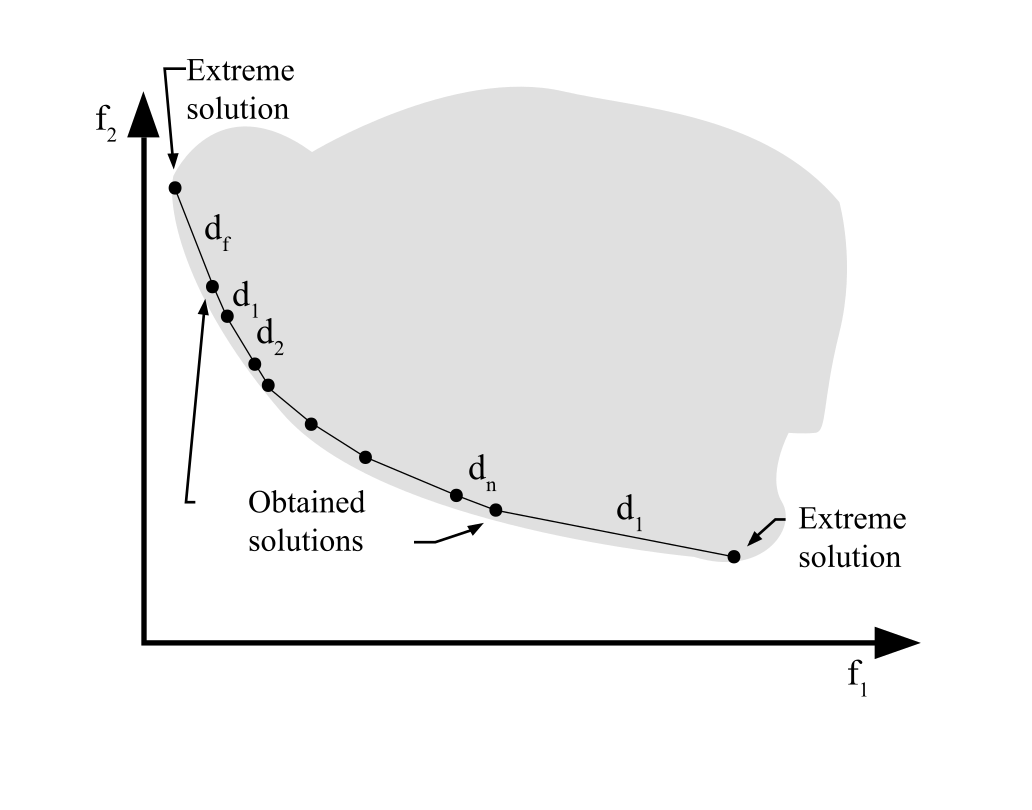
\includegraphics[width=0.5\textwidth]{images/spread_metric.png}
    \caption{Graph representing the Spread metric.}
    \label{fig:spread_graph}
\end{figure}

There may exist a scenario where are solutions lay within the same point, this is not considered the worst case of spread. When there is a great variance between the distance of the solutions the increment can be greater than one. On the other hand, a good distribution would make all the distances $d_i$ equal to the average $\overline{d}$, making $d_f$ and $d_t$ equal to zero, making $\bigtriangleup$ also zero. In the case of higher dimensions, a triangularization technique is used to calculate the distances for the solutions. \\

This metric was one of the most preferred in the literature. However, its usage has decreased in the recent years. One of the major drawbacks is that the metric alone only measures the diversity of the approximation to the Pareto front \cite{riquelme2015performance}. Nevertheless, combined with other convergence metric is still a relevant approach to assess the quality at a low computational cost. It should also be noted that it remains as the most popular metric to measure the diversity, but there is no more interest in the literature to measure the diversity alone to determine a quality set of solutions.

\subsection{Epsilon}

First defined in by Zitzler and Thiele in 2003 \cite{zitzler2003performance}. For a long time, it was considered the main indicator to describe the domination of the solutions \cite{riquelme2015performance}. It consists in getting a factor $\epsilon$ from which if an objective front are multiplied the Pareto front or any another front still dominates the former.\\

In the case of minimisation, a vector $\vec{z_{1}}$ is said to $\epsilon-$dominate another vector $\vec{z_{2}}$ if and only if for all the points of the vector $\vec{z_{2}}$ multiplied by a factor of $\epsilon$ remains higher than $\vec{z_{1}}$, this can be best described in Equation~\ref{epsilon_eq}.\\

\begin{equation} 
    I_{\in}(A,B) = \inf_{ \epsilon \in R} x \{\forall \vec{z_{2}} \in B \exists  \vec{z_{1}}  \in A: \vec{z_{1}} \succeq_{ \in } \vec{z_{3}}\}
    \label{epsilon_eq}
\end{equation} \\

Loosely speaking, a vector $\vect{z}$ is said to epsilon dominate another vector if the multiplication of each objective value in the other vector by a factor of e and the resulting objective vector is still weakly dominated by the first. The resulting Epsilon is the $E$ precise factor.\\

According to this the $\epsilon$-indicator gives the factor by which an approximation set is worse than another with respect to all its objectives, therefore $I_{\in}(A,B)$ equals to that minimum factor $\epsilon$ such that any objective in $B$ multiplied by the factor $\epsilon$ is $\epsilon$-dominated by at least one objective vector in $A$. For a single objective evaluation $I_{\in}(A, B)$ is simply the ratio between the two objectives $A$ and $B$.\\

\begin{figure}
    \centering
    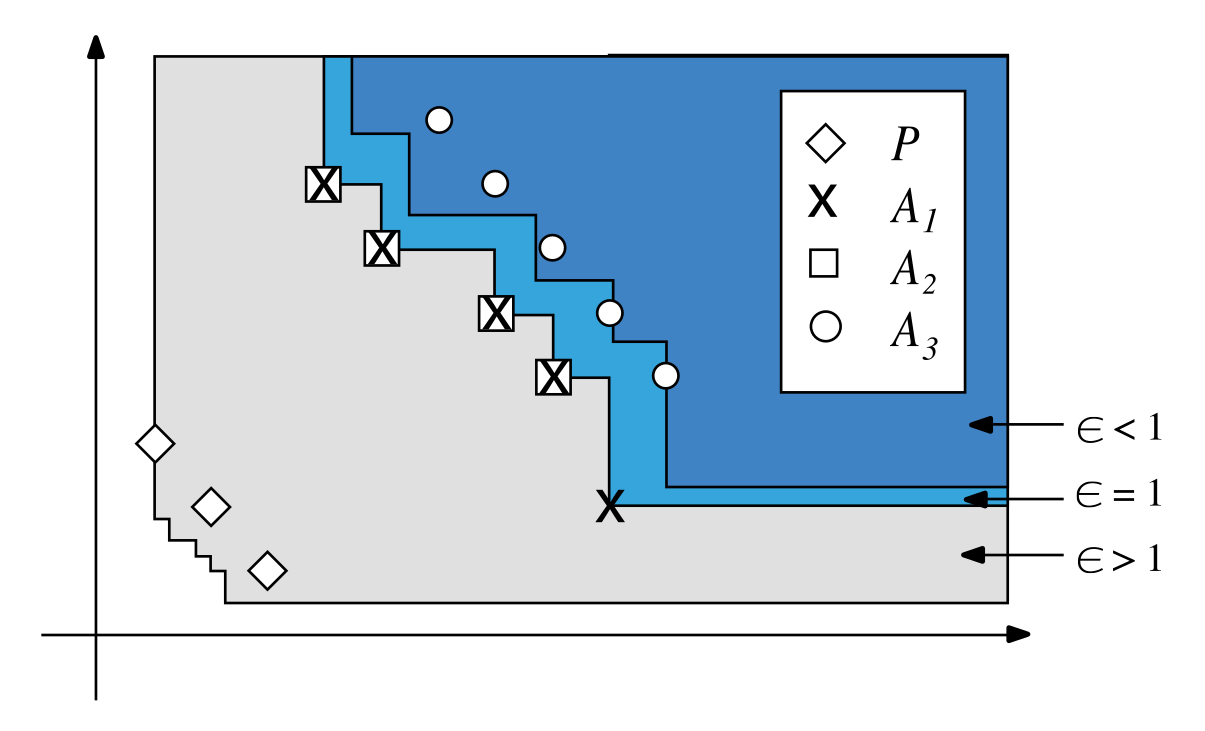
\includegraphics[width=\textwidth]{images/epsiolon.png}
    \caption{Graph representing the subspace of which Epsilon is based.}
    \label{fig:epsilon_graph}
\end{figure}

For example, in Figure~\ref{fig:epsilon_graph}, the dark blue area represents the subspace $\epsilon$-dominated by the solutions in $A_{1}$ for an $\epsilon = 9/10$, the light blue area refers to the subspace $\epsilon$-dominated by the solutions in $A_{1}$ for an an $\epsilon = 4$.

\subsection{Generational Distance}

Generational Distance (GD), was first used by Van Veldhuizen and Lamont in the early experiments done in 1998 \cite{van1998evolutionary}. GD is a value that consists in representing how far a known Pareto front is from the real Pareto front defined in Equation~\ref{eq:generational_distance}.

\begin{equation}
G \triangleq \frac{\left(\sum_{i=1}^{n} d_{i}^{p}\right)^{1 / p}}{n}
\label{eq:generational_distance}
\end{equation}

where $n$ is the number of solutions in the known Pareto front and $d_i$ is the Euclidean distance in the objective space between each of the solutions and the nearest member of the real Pareto front, and $p$ representing the number of objectives. When the known and the real Pareto front are the same the distance should be zero. Any other result shows how much the known Pareto Front deviates from the real one. \\

GD has been lowering its presence in the literature in recent years, as HV has been increasing is usage \cite{riquelme2015performance}. One of its main drawbacks in comparison to other metrics is that if a known front presents a large fluctuation in the distance values the calculated value may not represent the true distance.

\subsection{Inverted Generational Distance}

Inverted GD (IGD) \cite{coello2004study} can be calculated as the inverse of the GD starting with the Real Pareto Front and calculating the distance to the fronts produced by their tested algorithms \cite{ishibuchi2015study}. It can also be calculated by the following equation:

\begin{equation}
D\left(A, P^{*}\right)=\frac{\sum_{v \in P^{*}} d(v, A)}{\left|P^{*}\right|}
\end{equation}

Where $d(z_i,a_j)$ is the distance be a distance between $z_i$ and $a_j$ in the objective space. It is mentioned by \cite{zhang2007moea}, that If $|Z|$ is large enough to represent the Pareto Front well, then $D(A, P*)$ can be used to measure both the diversity and the convergence.\\

There are two main advantages of using IGD, the first is its computational efficiency even considering multi-objective problems with more than four objectives, called many-objective problems, especially comparing it to HV. The other is its generality, it usually shows the overall quality of an obtained front, considering its convergence and to it and its diversity. This is the main reason why its often used in the found literature \cite{7007204}.\\

However, besides the advantages gained from IGD it still has several disadvantages which are discussed in the following subsection.\\

\subsection{Inverted Generational Distance +}

While IGD is increasing its use, there are several disadvantages mentioned in \cite{ishibuchi2015study}, one of these known flaws, especially comparing it to the HV is its lack of Pareto compliant property, this can be further be seen in Figure~\ref{fig:igd_comp_1}

\begin{figure}[H]
    \centering
    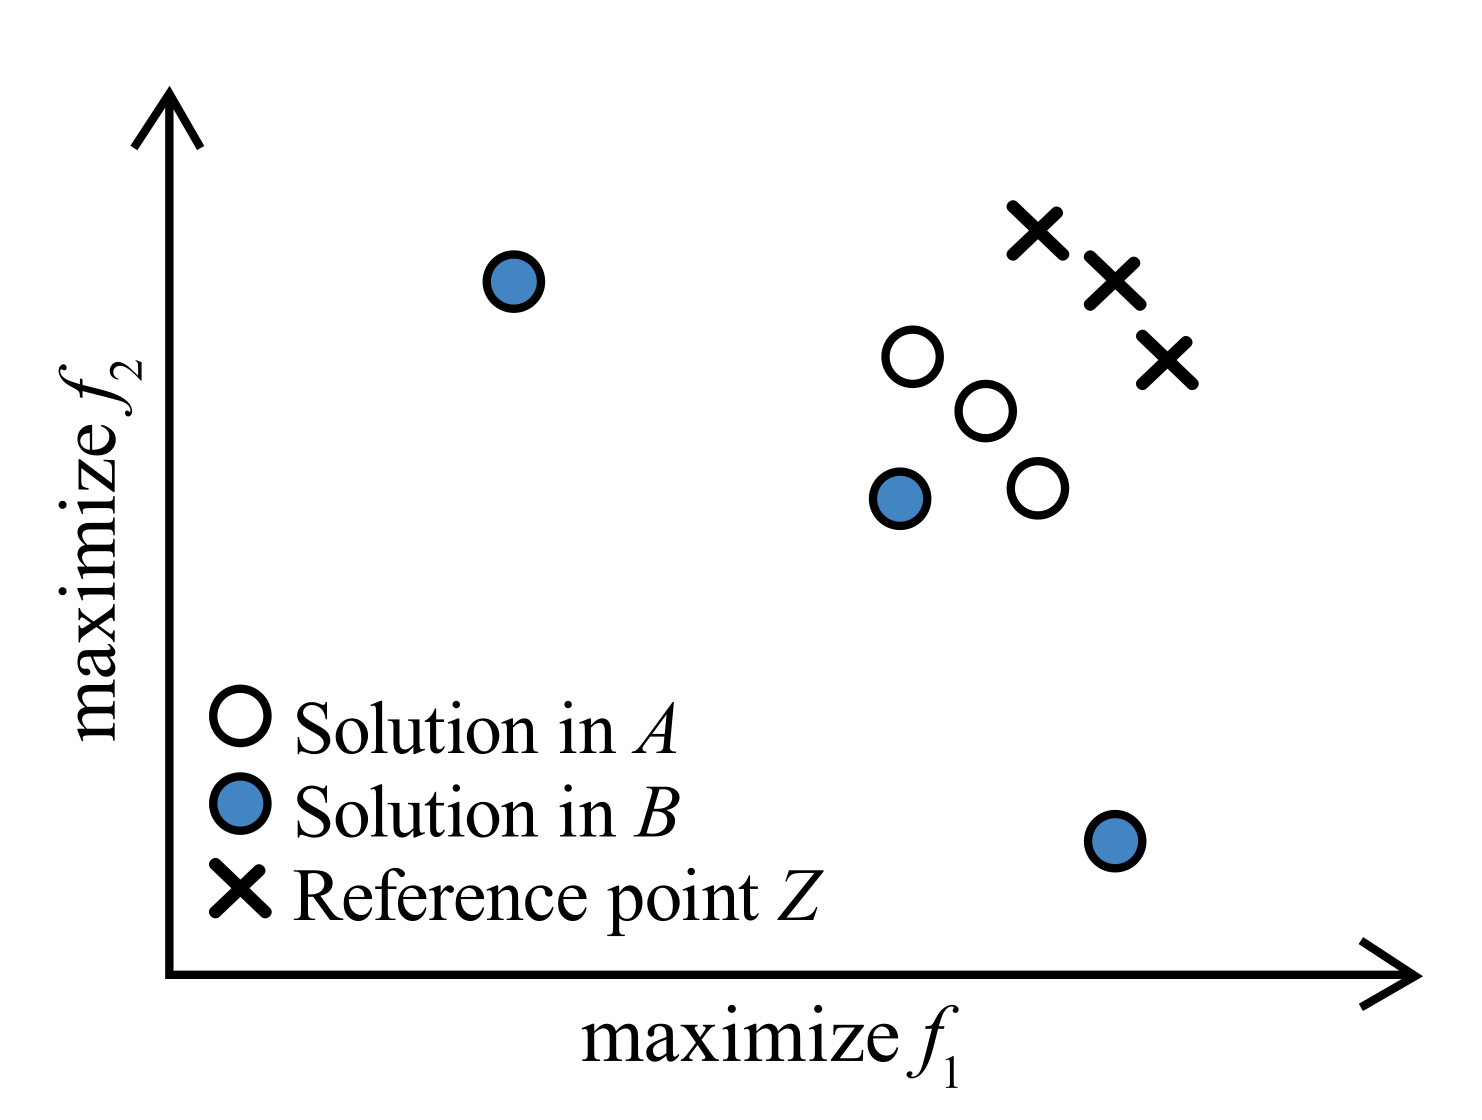
\includegraphics[width=0.5\textwidth]{images/igd_comp_1.png}
    \caption{Example of distance between Reference $Z$, Solution $A$ and Solution $B$.}
    \label{fig:igd_comp_1}
\end{figure}

\begin{figure}[H]
    \centering
    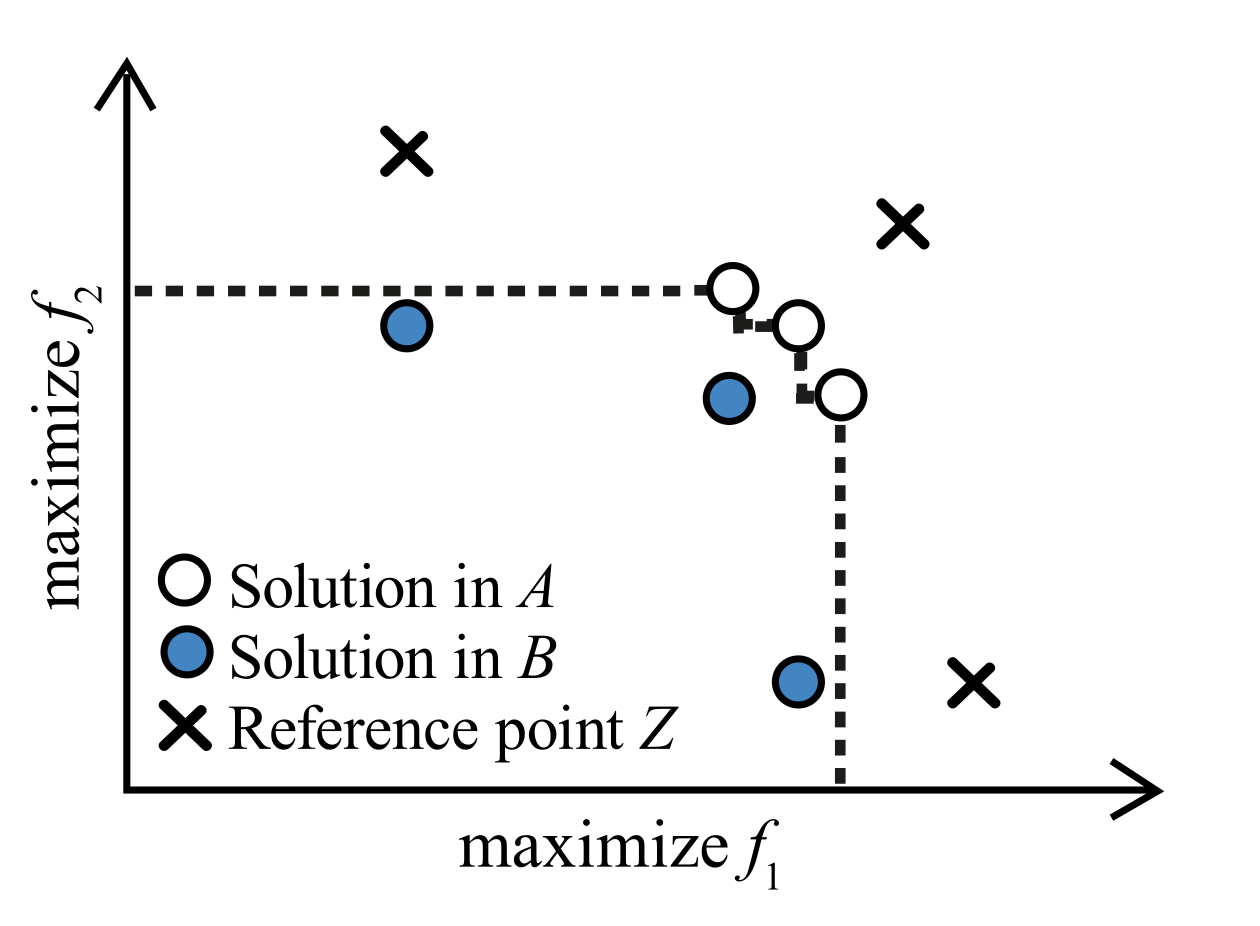
\includegraphics[width=0.5\textwidth]{images/igd_comp_2.png}
    \caption{Example of distance between Reference $Z$, Solution $A$ and Solution $B$, here the solutions from set $B$ appear to be closer to $Z$.}
    \label{fig:igd_comp_2}
\end{figure}

This presents a comparison between the front $A = (a_1, a_2, a_3)$ and the front $B = (b_1, b_2, b_3)$, and a reference Pareto front $Z = (z_1, z_2, z_3)$ for a maximisation problem. Here every solution in the front $B$ is clearly dominated by the solutions in the front $A$, however the measurement of IGD between $Z$ and $B$ would be lower, because of the way the solutions in $B$ are distributed which has a similar spread to $Z$.\\

To address these drawbacks, IGD+ was proposed by Ishibuchi and Masuda~\cite{ishibuchi2015study}. It is closely similar to IGD with the difference of having a weak Pareto compliant property, and it is based on the idea of calculating the distance from each reference point to a dominated region instead of the nearest solution, this can be seen in Figure~\ref{fig:igd_comp_3}.\\

Then, ($IGD+$) is defined as the distance between a Pareto front $Z$ and a solution front $A$.

\begin{figure}[H]
    \centering
    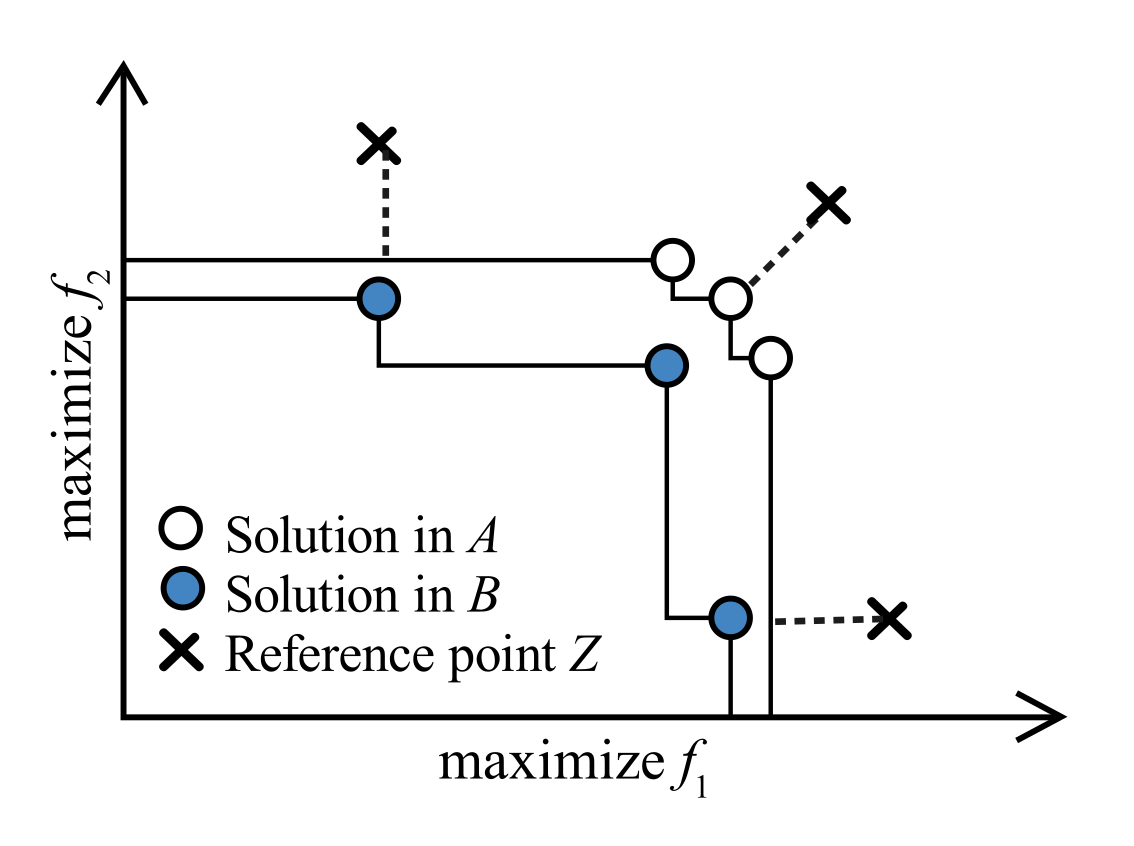
\includegraphics[width=0.5\textwidth]{images/igd_comp_3.png}
    \caption{A graph representing the main idea behind ($IGD+$).}
    \label{fig:igd_comp_3}
\end{figure}

Here, if a solution $A$ is dominated by the reference front $Z$, then $d_{IGD+}(A,Z)$ is the same as the euclidean distance $d(A,Z)$, because all the solutions in the front $A$ are smaller than those from the reference front $Z$, and this also holds for each point in their respective fronts. When $A$ and $Z$ are not dominated with each other, only the objectives in $A$ that are lower to their counterparts in $Z$ are used, which means that if a point in the front $A$ is better than another from point $Z$ with respect to some of its objective, then these are not used in the calculation of IGD+.\\

\section{Frameworks}
\subsection{jMetal}

jMetal is a framework based on the Java programming language. It is focused on development, experimentation and study of meta-heuristics to solve MOPs. JMetal includes various of the most common algorithms. A series of example problems and regularly used indicators to measure the performance of algorithms. It also includes tools to carry out experimental studies that can be configured to generate statistical reports of the obtained results. It is also possible to take advantage of a multi-core architecture to make the experimentation process faster~\cite{durillo2011jmetal}.\\

Some of the features sought are part of this type of software are:

\begin{itemize}
    \item Include the most current algorithms available
    \item Contain the most accepted performance tests for multi-objective problem solving
    \item Give quality indicators to measure the performance of each of the tests and assist in a more accessible way in the investigations of its users.
\end{itemize}

\subsection{James}

 James, which stands for Java Metaheuristics Search, is an object‐oriented Java framework for discrete optimisation using local search algorithms that takes advantage of the generality of such meta-heuristics by separating search implementation and application from each problem specification. A wide range of generic local searches is provided, including:
 (Stochastic) Hill climbing, Tabu search, Variable neighbourhood Search and Parallel Tempering. These can be applied to any user‐defined problem by designing a custom neighbourhood for the corresponding solution type. Using an automated analysis workflow, the performance of different search algorithms can be compared to select an appropriate optimisation strategy \cite{de2017james}.\\
 
 Implementations of specific components are included for subset selection, such as a predefined solution type, generic problem definition and several subset neighbourhoods used to modify the set of selected items. In comparison with existing Java meta-heuristics frameworks that mainly focus on population‐based algorithms, JAMES has a much lower memory footprint and promotes the efficient application of local searches by taking full advantage of move‐based evaluation and parallelization.\\

\section{Preference Criteria}
\label{section:preference_criteria}

This section describes the different metrics used as a basis for the objective functions based on the predicted preference of the students according to the group they want to belong.

\subsection{Benne and Sheats functional roles}
\label{section:functional_roles}
The Benne and Sheats functional roles are a tool that helps define what kind of reaction a person has at the time of starting a conversation \cite{benne2007functional}. The roles we are specifically interested in are known as the \textbf{Maintenance Roles}.

\begin{itemize} 
    \item \textbf{Attacker}: Is that person who invalidates the comments of others and "attacks" the rest of the group members.
    \item \textbf{Protagonist}: is the person who initiates the conversations, assumes an authority role. In this case, it is a very valuable role in our research.
    \item \textbf {Follower (or Supporter)}: This person has a cooperative attitude, pays attention to the talk, accepts the proposals and offers technical support.
    \item \textbf{Gatekeeper}: is a person who plays the role of moderator, checking that each person has their opportunity to participate similarly.
    \item \textbf{Neutral}: It is similar to the follower role, only instead of actively participating, it accepts the comments passively.
\end{itemize}

It should be noted that a person can represent different types of roles in the same conversation, although it is generally classified depending on which was their most prominent role.

\subsubsection{AMI Meeting Corpus}

AMI meeting corpus is a data-set containing the recording of several conversations in different contexts. With the purpose to analyse the interaction between the participants. It has been used in several works to predict participation styles such as Vinciarelli \cite{VinciarelliUnderstandingCorpus} who uses this database to identify the functional roles of Benne and Sheats \cite{benne2007functional}.

\subsection{Facebook Ad Platform}
\label{section:facebook_ad_platform}

The social network known as Facebook is useful to maintain contact between friends and acquaintances, however, it is also a useful marketing tool to give users who belong to certain market ads focused on each of them according to their preferences, behaviours and locations. This follows a marketing methodology known as Demography, Behaviours and Interests. As far as this research is concerned, we are only interested in the Interests.\\

These interests are determined by the classification of the pages or groups that the user follows, however it has a more general classification as an ontology that Facebook has been building over the years using different clustering techniques so that It can have a more general categorisation of the different types of interests of each of the users.\\

Besides, Facebook allows businesses through a platform known as \textbf{Facebook ad Platform} \cite{facebook_business} publish different types of ads aimed at a type of market according to the interests or behaviours corresponding to a market. This platform is public and can be used to determine an approximate cost when preparing marketing campaigns. However, this research is used to determine the population size for each of the interests described as it will be mentioned in Sections \ref{chapter:chapter03} and \ref{chapter:chapter04}.\\

This platform can also be used at the same time to generate the distribution of the data since it is directly linked to the ontology and can be consulted to measure the distances between one interest and another. Part of the ontology can be seen in Figure~\ref{fig:facebook_ontology_02}.\\

\begin{figure}
    \centering
    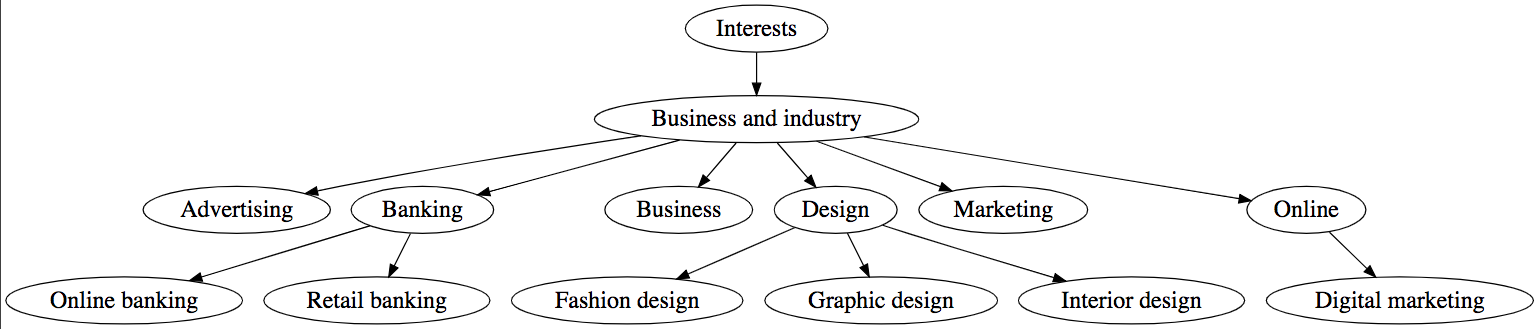
\includegraphics[width=150mm]{ontology.png}
    \caption {An example of the Facebook interests ontology.}
    \label{fig:facebook_ontology_02}
\end{figure}

The ontology that Facebook has created is determined with a tree of 8 general and 314 specific interests. Each classified according to the relation to the general interest. This allows to search for specific interests in common, for example, if a person likes television programs we can also assume that she may also like reality shows or contest programs etc. In this way, another person who has an interest in television series has a direct relationship with the first. On the other hand, interests that have no relation, have no connection in the ontology.\\

% It may also be important to explain the ontology by indicating its parts and how the interest of a branch may be related to one in another branch

\subsection{CEFR}

Known as \textbf{Common European Framework of Reference for Languages} for its acronym in English, it is a tool used internationally to assess the level of knowledge of a foreign language and is commonly known throughout the world in such a way that although a different test has been performed, it is possible to find a type of equivalence using this classification, which allows being able to take into account at the level of a person regardless of what type of test taken.\\ 

The levels are classified as A1, A2, B1, B2, C1 and C2. The first two levels, A1 and A2, refer to the most basic levels where a person knows the basics of the language, such as introduce themselves or asking for directions. The second tier, B1 and B2 are considered the intermediate level, people in this classification can understand long casual conversations as well as writing and reading non-specialised content. The last two levels C1 and C2 refer to people with the ability to deeply understand and speak the language, moreover, to write full documents using it.
